\documentclass[12pt]{SeminarskiADS}

\begin{document}
\Predmet{Adaptivni diskretni sistemi i neuralne mreže}
\Nastavnik{Prof. dr Miloš Daković}
\Naslov{Obrada EKG signala pomoću LMS algoritma i klasifikacija pomoću SVM klasifikatora}
\Kandidat{Andrej Jokić}
\Indeks{19/2018}
\Datum{januar 2019.}
\maketitle 


\section{Uvod}
Elektrokardiografija je veoma značajna u dijagnozi mnogih srčanih poremećaja. Elektrokardiogram (EKG) je grafički prikaz električne aktivnosti srca. Na njemu su prikazane promjene bioelektričnog potencijala u vremenu. Mnogi poremećaji u radu srca se mogu uočiti analizom oblika EKG signala i varijacije pulsa (\emph{HRV - Heart Rate Variation}) \cite{gl}. 

Jedan od široko rasprostranjenih srčanih poremećaja je aritmija (poremećaj srčanog ritma). Aritmija obuhvata više srčanih bolesti kod kojih su otkucaji srca nepravilni, prespori ili pak prebrzi \cite{what_is_arr}. Ovakvi poremećaji se dosta pouzdano mogu otkriti analizom EKG snimka. Kako biosignali nisu stacionarni, indikacije ovog poremećaja se mogu pojaviti u nasumičnim trenucima. Naime, simptomi aritmije često nisu prisutni sve vrijeme, već se pojavljuju u nepravilnim intervalima u toku dana. Stoga, radi efektivne dijagnoze, EKG se ponekad snima i po nekoliko sati. Analiza ovako velike količine podataka je teška i oduzima mnogo vremena. Takođe, postoji mogućnost da ljekar ne uoči ili pogrešno protumači neki značajan podatak. Zbog toga se dosta radi na razvoju računarskih tehnika za analizu EKG snimaka \cite{ecg_multiclass_svm}.

U toku snimanja i prenosa, EKG signali često bivaju zahvaćeni određenom količinom šuma. Prisustvo šuma može otežati analizu ili prouzrokovati pogrešno tumačenje podataka. Zato je prije analize potrebno filtrirati signal kako bi se uklonilo što više šuma. Neke od tehnika filtriranja koje se koriste za EKG signal su IIR notch filtri, FIR filtri, adaptivni filtri, Wavelet transformacija itd. \cite{ecg_denoise} U ovom radu ćemo primijeniti adaptivni filtar zasnovan na LMS algoritmu. 

Kako bi se signali efektivno klasifikovali, potrebno je izdvojiti određena svojstva ovog signala. SVM klasifikator će na osnovu ovih svojstava svrstati signale u odgovarajuće klase. EKG signali sadrže značajne podatke i u vremenskom i u frekvencijskom domenu. Zato se za izdvajanje svojstava EKG signala često koristi diskretna wavelet transformacija. DWT omogućava da se ogromna količina podataka koja karakteriše EKG signal komprimuje u mali broj značajnih parametara. 


%Nesto da se u poslednjim godinama mnogo posvecuje paznja razvoju tehnika masinskog ucenja za 
Mašinsko učenje omogućava računaru da analizom velike količine podataka ``uoči'' veze između pojedinih elemenata. Mnogi naučni radovi istražuju primjenu različitih algoritama mašinskog učenja u klasifikaciji EKG signala. Neke od tehnika koje se primjenjuju su KNN (\emph{K-Nearest-Neighbor}), \emph{Neuro Fuzzy} klasifikator, SVM (\emph{Support Vector Machine}), \emph{Deep Learning} itd. Rezultati su pokazali da najbolje performanse i najveću tačnost klasifikacije EKG signala ima SVM klasifikator. 

%Visokofrekventni šumovi kod EKG signala najčešće obuhvataju bijeli gausov šum i sinusoidalne smetnje iz električne mreže. 

\section{EKG}

Za dobro funkcionisanje kardiovaskularnog sistema, neophodno je da se srčani mišići kontrahuju u pravilnom ritmu. Ritam kontrakcija srčanog mišića kontrolišu električni impulsi koji potiču iz \emph{sinusnog čvora} (\emph{P ćelije}). Dio struja prouzrokovanih električnim impulsima stiže do površine kože, gdje izazivaju promjene električnog potencijala. Elektrokardiograf je zapravo precizan galvanometar koji mjeri ove potencijale. Kod standardnog EKG-a, na tijelo pacijenta se postavlja 12 elektroda, koje mjere razlike potencijala između određenih tačaka na površini kože.

Na slici \ref{ecg_otkucaj} je prikazan jedan otkucaj srca na EKG snimku kod zdrave osobe (normalni sinusni ritam). Jedan otkucaj se sastoji iz P talasa, QRS kompleksa i T talasa. Za analizu varijacije pulsa (HRV) najznačajnija je detekcija QRS kompleksa, tj. detekcija R pika. Automatska detekcija R-pikova nije jednostavna, kako zbog fiziološke varijabilnosti QRS kompleksa, tako i zbog prisustva raznih šumova i smetnji u EKG signalu \cite{rpeak_dwt}. Postoje mnogi softverski paketi za detekciju R pikova i HRV analizu. U ovom radu je korišćen open-source toolbox za \emph{Matlab} softverski paket, ``Physionet Cardiovascular Signal Toolbox'' \cite{physionet_tbx}. Primjeri EKG signala su preuzeti iz opšteprihvaćene MIT-BIH baze. Uz same EKG signale, u ovoj bazi su dostupni i ručno obilježeni R-pikovi \cite{mit_bih}. %TODO dodaj koje signale si preuzeo i koliko njih, dužina, Fs...




%sto je ekg

%qrs

%slika qrs

\begin{figure}[h]
\centering
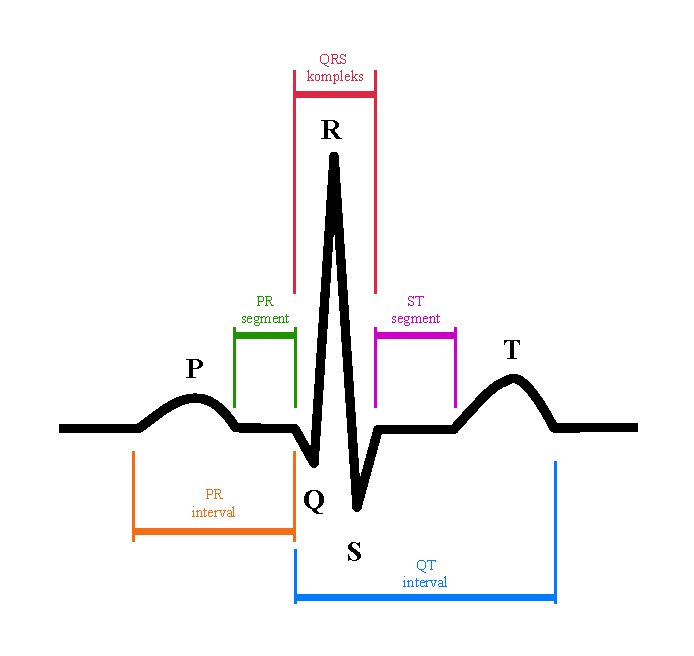
\includegraphics[width=0.8\textwidth]{ecg_otkucaj}
\caption{Jedan otkucaj srca na EKG snimku}
\label{ecg_otkucaj}
\end{figure}


\section{LMS filtriranje}
\label{sec:lms}

EKG signali su obično zahvaćeni određenom količinom šuma koji nastaje u toku snimanja ili prenosa signala. Uglavnom su zastupljene dvije vrste šuma. Visokofrekventni šumovi obuhvataju sinusoidalne smetnje iz električne mreže (50/60Hz), kao i šum koji nastaje usljed nesavršenosti samog uređaja za snimanje. Niskofrekventni šum koji je prisutan kod EKG signala naziva se \emph{baseline wander}. Ovaj šum nastaje kao posljedica fizičkog pomjeranja tijela pacijenta (disanje ili slučajni pokreti) \cite{ecg_denoise}. Takođe, ako se EKG signal prenosi bežičnom vezom, prisutan je i kanalni šum. Ovaj šum takođe ima karakteristike bijelog Gausovog šuma. Većina šumova koji su prisutni mogu se modelovati bijelim gausovim šumom \cite{gl}.

Prisustvo veće količine šuma značajno utiče na oblik EKG signala. Ovo može izazvati pogrešno tumačenje podataka i grešku u klasifikaciji. Prema tome, potrebno je izvršiti obradu signala kako bi se uklonila što veća količina šuma prije računanja parametara i klasifikacije. Usljed promjenljive prirode EKG signala, uklanjanje šuma iz EKG signala nije jednostavno. Neke od tehnika koje se koriste su IIR notch filtri (za uklanjanje sinusoidalnih smetnji), \emph{Wavelet Transform Thresholding}, \emph{Bionic Wavelet Transform}, adaptivni filtri. Adaptivno filtriranje podrazumijeva upotrebu LMS, RLS ili EMD (\emph{Empirical Mode Decomposition}) algoritama. Tehnike zasnovane na wavelet transformaciji, kao i na RLS i EMD algoritmima su računski veoma zahtjevne \cite{gl}. U ovom radu će biti primijenjeno filtriranje pomoću LMS algoritma.

\begin{figure}[h]
\centering
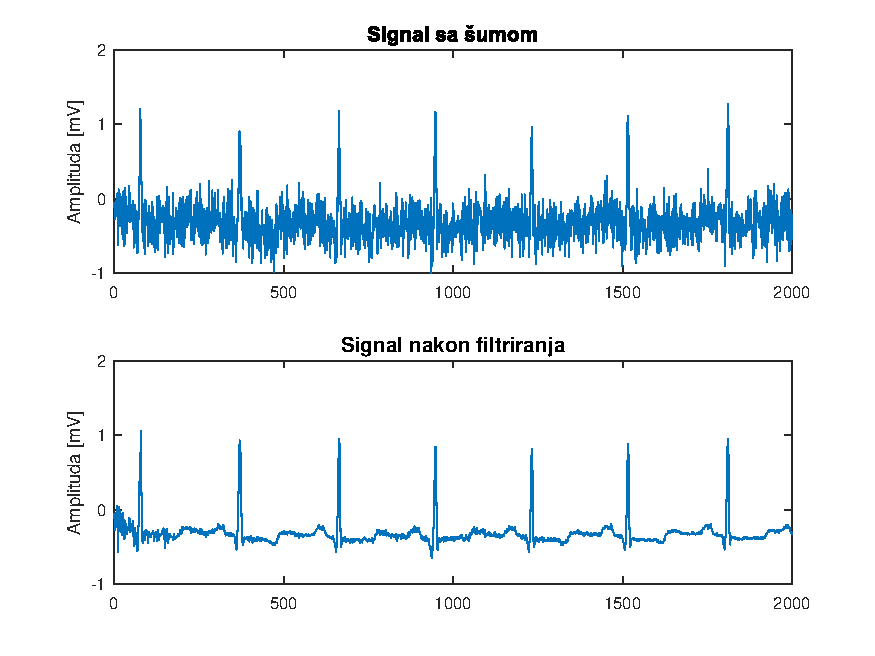
\includegraphics[width=\textwidth]{lmsgrafik}
\caption{Signal prije i nakon filtriranja}
\label{lmsgrafik}
\end{figure}

LMS algoritam je veoma efikasan u odnosu na ostale adaptivne metode filtriranja. U prenosnim medicninskim uređajima primjena ovog algoritma omogućava upotrebu jednostavnijeg hardvera i manju potrošnju električne energije. Takođe, ovaj algoritam ima dobre performanse uklanjanja šuma kod vremenski promjenljivih signala. 

Na slici \ref{lmsgrafik} je prikazan primjer primjene adaptivnog filtriranja. Na gornjem grafiku je prikazan jedan signal iz MIT-BIH baze kome je dodat bijeli gausov šum. Primjenom adaptivnog filtra prema slici \ref{lms_denoise} (tako da zašumljeni signal predstavlja \verb|d(n)|, a sami šum je \verb|x(n)|), dobija se signal koji je prikazan na donjem grafiku. Uočava se da šum onemogućava prepoznavanje oblika signala, naročito P i T talasa (R talas se i dalje može uočiti).

Za dobijanje ovog rezultata primijenjen je \emph{normalizovani LMS} algoritam. Za razliku od običnog LMS-a, u ovom algoritmu se korak $\mu$ u svakoj iteraciji mijenja po formuli:

\begin{equation}
\label{eq:nlms}
\mu=\frac{\mu_{0}}{1+X^T(n)X(n)}.
\end{equation}  

gdje $\mu_{0}$ predstavlja osnovnu vrijednost koraka.

Kako bi se postigao što brži odziv, pored normalizacije, u ovom algoritmu je primijenjen i varijabilni korak. Početna vrijednost $\mu_{0}$ je postavljena na 1, kako bi se koeficijenti filtra što brže približili optimalnim vrijednostima. Nakon $200$ odbiraka, korak je smanjen na $0.10$, a nakon $700$ odbiraka na $0.05$, kako bi se koeficijenti mogli što preciznije prilagoditi signalu. Na ovaj način se u prosjeku postižu odlične performanse filtriranja već nakon 200 odbiraka.

Radi poređenja, na slici \ref{lmsgrafik_por} prikazan je isti signal filtriran pomoću tri različite varijante LMS algoritma. Na prvom grafiku je prikazan LMS algoritam sa fiksnim korakom, na drugom normalizovani LMS, a na trećem normalizovani LMS sa postepenim smanjivanjem koraka. Može se uočiti da obični i normalizovani LMS imaju približno iste performanse u ovom slučaju. Međutim, normalizovani LMS se može bolje prilagoditi na promjene intenziteta šuma koje se mogu javiti u realnim situacijama. Najbolje performanse se uočavaju kod NLMS algoritma sa postepenim smanjivanjem koraka. Veliki početni korak omogućava filtru da se veoma brzo prilagodi signalu, u ovom slučaju već nakon 100 odbiraka. Kada se koeficijenti filtra približe optimalnim vrijednostima, mali korak omogućava precizno podešavanje koeficijenata i veoma dobro filtriranje u svim djelovima signala. 

\begin{figure}[h]
\centering
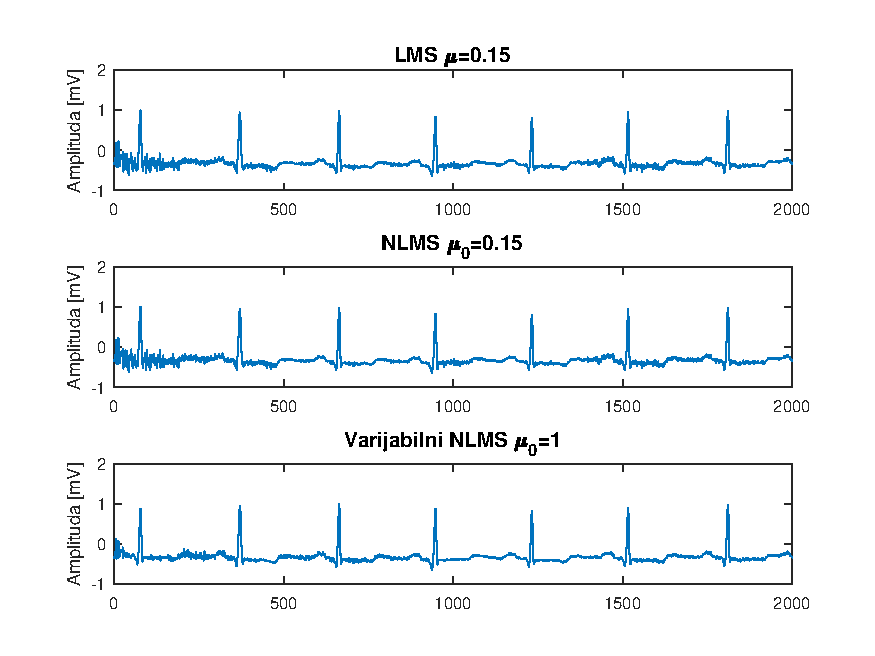
\includegraphics[width=\textwidth]{lmsgrafik_por}
\caption{Poređenje različitih varijanti LMS algoritma}
\label{lmsgrafik_por}
\end{figure}


\begin{figure}[tbp]
\centering
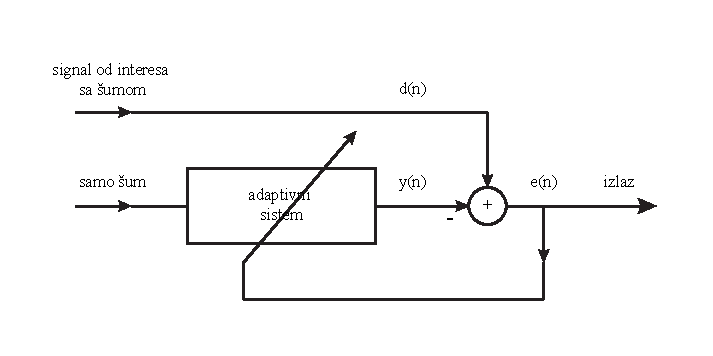
\includegraphics[width=0.9\textwidth]{lms_denoise}
\caption{Adaptivni sistem za uklanjanje šuma}
\label{lms_denoise}
\end{figure}

\section{Izdvajanje svojstava}
\label{sec:extraction}
%TODO jos prije ovoga
Kod klasifikacije pomoću mašinskog učenja, veoma veliki značaj ima izdvajanje svojstava signala (eng. \emph{feature extraction}). Ovo podrazumijeva proces izbora i računanja određenih parametara koji što bolje opisuju dati signal i koji ga razlikuju od signala iz ostalih klasa. U većini realnih situacija, signal koji obrađujemo sadrži ogromnu količinu podataka. Veliki dio ovih podataka nije značajan za datu klasifikaciju, ili više podataka nosi jednu značajnu informaciju. Obrada velike količine podataka je veoma neefikasna jer se mnogo resursa troši bez potrebe. Takođe, kako klasifikator pokušava da pronađe značajne veze između podataka, prisustvo beskorisnih informacija rezultira izvođenjem pogrešnih zaključaka i zahtijeva mnogo više treniranja kako bi se postigla željena preciznost klasifikacije. Prema tome, izbor što manjeg broja kvalitetnih svojstava direktno utiče na performanse i preciznost klasifikacije \cite{feat}. 

Izdvajanje svojstava je veoma široka naučna oblast i može se izvršiti na mnogo načina. U ovom radu će biti predstavljena dva pristupa za izdvajanje svojstava iz EKG signala. Osnovni zadatak klasifikatora koji će biti predstavljen je razlikovanje signala koji predstavljaju normalni sinusni ritam (NSR) od signala koji pokazuju svojstva aritmije (ARR).

Kao što je pomenuto, aritmija predstavlja skup srčanih bolesti koje karakteriše srčanog ritma. Može se zaključiti da su najznačajnije informacije za detekciju ovakvog poremećaja sadržane u samom srčanom ritmu. Prema tome, prvi pristup izdvajanju svojstava će se temeljiti na analizi varijacije pulsa (HRV - Heart Rate Variation). HRV analiza obuhvata skup metoda za računanje parametara koji opisuju srčani ritam u vremenskom i frekvencijskom domenu. Neki od dobro poznatih parametara su: 
\begin{itemize}
\item \textbf{Parametri u vremenskom domenu: } RR mean, RR std, HR mean, HR std, RMSSD, NN50, pNN50, RR trougaoni indeks i TINN.
\item \textbf{Parametri u frekvencijskom domenu: } VLF snaga, LF snaga, HF snaga, LF norma, HF norma i odnos LF/HF.
\end{itemize}
Pokazuje se da su ovi parametri veoma pogodni za detekciju aritmije \cite{gl}. Dostupno je više alata za računanje ovih parametara. Jedan od njih je National Instruments Biomedical Toolkit, koji dodatak za komercijalni softverski paket LabView. Alternativa ovom alatu je third-party open-source paket za Matlab pod nazivom PhysioNet Cardiovascular Signal Toolbox \cite{physionet_tbx}. 

%prvo napisem koji sumovi zahvataju signal, kako uticu na filtriranje

%onda primjenu LMS algoritma za uklanjanje suma

%slika lms denoising i denlms

%NLMS i DENLMS

%prikaz rezultata


\clearpage
\begin{thebibliography}{99}
\bibitem{gl} C. Venkatesan, P. Karthigaikumar, Anand Paul, S. Satheeskumaran, R. Kumar, ``ECG Signal Preprocessing and SVM Classifier Based Abnormality Detection in Remote Healthcare Applications'', IEEE Access, 2018.

\bibitem{what_is_arr} National Heart, Lung, and Blood Institute, ``What is arrhythmia?''
\url{https://www.nhlbi.nih.gov/health-topics/arrhythmia}

\bibitem{ecg_multiclass_svm} Elif Derya Übeyli, ``ECG beats classification using multiclass support vector machines with error correcting output codes'', Digital Signal Processing, 2007.

\bibitem{ecg_denoise} Aswathy Velayudhan, Soniya Peter, ``Noise Analysis and Different Denoising Techniques of ECG Signal - A Survey'', IOSR-JECE, 2016.

\bibitem{dsp} Ljubiša Stanković, ``Digital Signal Processing''

\bibitem{rpeak_dwt} K. Deergha Rao, ``DWT Based Detection of R-peaks and Data Compression of ECG Signals'', IETE Journal of Research, 1997.

\bibitem{physionet_tbx} Vest A, Da Poian G, Li Q, Liu C, Nemati S, Shah A, Clifford GD, ``An Open Source Benchmarked Toolbox for Cardiovascular Waveform and Interval Analysis'', Physiological Measurement (In Press), DOI:10.5281/zenodo.1243111, 2018.

\bibitem{mit_bih} Moody GB, Mark RG, ``The impact of the MIT-BIH Arrhythmia Database'', IEEE Eng in Med and Biol 20(3):45-50, May-June 2001 (PMID: 11446209). 

\bibitem{feat} Isabelle Guyon, ``Feature Extraction: Foundations and Applications'', Pattern Recognition, Springer, 2006.

\end{thebibliography}


\end{document}
